%文章初始设置----------------------------------------------------------------------------------------------------------------
\documentclass[12pt,a4paper,oneside,UTF8]{ctexart}
\usepackage{amsmath, amsthm, amssymb}
\usepackage[T1]{fontenc}
\usepackage{authblk}
\usepackage{listings}
\usepackage[usenames,dvipsnames]{xcolor}

\usepackage{graphicx, float}
\graphicspath{ {./PNG_files} }

\usepackage[ruled,linesnumbered,lined,boxed,linesnumbered]{algorithm2e}

\setmainfont{Times New Roman}
\usepackage{xeCJK}
\setCJKmainfont[AutoFakeBold,AutoFakeSlant]{SimSun}
\ctexset{
	section={aftername=\hspace{1em},format=\heiti\centering\zihao{3}\mdseries, afterskip=0bp,beforeskip=0bp,},% 设置 section 标题为黑体、右对齐、小4号字
	subsection={aftername=\hspace{0.5em},format=\heiti\raggedright\zihao{-3}, afterskip=0bp,beforeskip=16bp,},% 设置 subsection 标题为黑体、5号字
	subsubsection={format=\heiti\raggedright\zihao{4}, aftername=\hspace{0.5em},afterskip=0bp,beforeskip=0bp},% 设置 subsubsection 标题为黑体、5号字
	paragraph={format=\Simsun\raggedright\zihao{-4}, aftername=\hspace{0.5em},afterskip=0bp,beforeskip=0bp}
}

\renewcommand*{\Affilfont}{\small\it}
\renewcommand\Authands{ 与 }

\newcommand{\enabstractname}{Abstract}
\newenvironment{enabstract}{
  \addcontentsline{toc}{section}{Abstract}
  \par\small
  \noindent\mbox{}\hfill{\bfseries\small \enabstractname}\hfill\mbox{}\par
  \vskip 2.5ex}{\par\vskip 2.5ex}

\newcommand\cnkeywords[1]{\par\noindent{\heiti 关键字}: #1}
\newcommand\enkeywords[1]{\par\noindent\textbf{Keywords}: #1}

\makeatletter
\renewcommand\@biblabel[1]{[#1]\hfill}
\makeatother
\renewcommand\refname{}

% 定义颜色
\definecolor{mygreen}{rgb}{0,0.6,0}
\definecolor{mygray}{rgb}{0.5,0.5,0.5}
\definecolor{mymauve}{rgb}{0.58,0,0.82}

% 设置代码样式
\lstset{
  language=C++, % 指定语言
  basicstyle=\ttfamily\small, % 基本字体样式
  keywordstyle=\color{blue}, % 关键字颜色
  commentstyle=\color{mygreen}, % 注释颜色
  stringstyle=\color{mymauve}, % 字符串颜色
  numbers=left, % 显示行号
  numberstyle=\tiny\color{mygray}, % 行号样式
  frame=single, % 添加边框
  breaklines=true, % 自动换行
  tabsize=4 % Tab 宽度
}

%标题区----------------------------------------------------------------------------------------------------------------
\title{《无人机摄像及应用》结课报告\\航迹规划算法与实现}
\author[1]{刘宇轩}
\author[2]{李顺龙}
\author[2]{郭亚鹏}
\author[2]{王安东}
\author[1]{刘一诺}
\author[1]{何家震}
\author[1]{齐露雅}
\author[1]{石艾琳}
\author[1]{张芮嘉}

\affil[1]{哈尔滨工业大学\ 《无人机摄像及应用》(TS22505)2025秋季班\  第三组}
\affil[2]{哈尔滨工业大学\  交通科学与工程学院\  桥梁结构安全评定青年科学家工作室,\qquad 黑龙江\ 哈尔滨\ 150001}
\affil[*]{班级、学号等信息请见文后致谢部分}
\date{}

%内容区----------------------------------------------------------------------------------------------------------------
\begin{document}
%封面--------------------------------------------------------
\pagestyle{empty}\maketitle\thispagestyle{empty}
%摘要--------------------------------------------------------
\newpage\setcounter{page}{1}\pagenumbering{Roman}\pagestyle{plain}\begin{abstract}
    \addcontentsline{toc}{section}{摘要}
    在全球桥梁数目与规模逐渐增大的背景下,
    传统的纯人力方式与手动操控无人机方法已经难以维持多种工作进行。
    因此,
    引入自动化控制的无人机飞行工作已经成为共识。

    而航迹规划是无人机自动控制中必不可少的一环,
    就此,
    本文将对航迹规划问题进行以下研究操作:
    
    (一)航迹图图形化或栅格化。

    (二)使用多种路线规划算法对多种给定飞行情形进行自动航线规划,
    包括基于图的传统基本航迹规划算法,
    例如模拟算法,迪杰斯特拉算法(Dijkstra)和IDA*搜索算法,
    以及基于机器学习的现代智能路线规划算法,
    例如遗传算法、蚁群算法(Ant Colony Optimization, ACO)、灰狼优化算法(Grey Wolf Optimizer, IGWO)和布谷鸟搜索算法(Cuckoo Search, CS),
    以满足不同现实情境下的不同工作需求。

    (三)利用航迹平滑算法,
    包括三次样条插值法(Cubic Spline Interpolation, Spline插值)和贝塞尔曲线法(Bézier Curve)算法,
    对航迹进行实际航迹可行化处理。


\end{abstract}
\cnkeywords{无人机,航迹规划,规划算法,最优化问题}
\newpage\begin{enabstract}
    Against the backdrop of a continuous increase in the number and scale of bridges worldwide, 
    traditional manual approaches and manual drone operation methods have proven inadequate to sustain a wide range of tasks.
    As such, 
    the introduction of automated drone flight operations has become widely acknowledged.
    And path planning is an essential component of autonomous drone control.  
    In this regard,  
    this paper will conduct the following research on the path planning issue:  

    (1) Graphical or grid-based representation of path maps.  

    (2) Utilization of various route planning algorithms for automated route planning under multiple given flight scenarios,  
    including traditional graph-based fundamental path planning algorithms,  
    such as simulation algorithms, Dijkstra's algorithm, and IDA* search algorithm,  
    as well as modern intelligent route planning algorithms based on machine learning,  
    such as genetic algorithms, ant colony optimization, grey wolf optimization algorithms, and cuckoo search algorithms,  
    to meet different operational requirements in various real-world situations.  

    (3) Application of path smoothing algorithms,  
    including the cubic spline interpolation method and the Bézier curve algorithm,  
    to ensure the feasibility of paths in practical flight operations.
\end{enabstract}
\enkeywords{UAV, Flight path planning, Planning algorithm, Optimization problem}
%目录--------------------------------------------------------
\newpage\pagestyle{plain}
\tableofcontents
%正文--------------------------------------------------------

%绪论-------------------------
\newpage\setcounter{page}{1}\pagenumbering{arabic}\section{绪论}
截至2025年末,
我国公路桥梁数量已经超过110.81万座\textsuperscript{\cite{ref1}}。
桥梁正式投用后,
因服役年限的增加与自然因素的损耗,
使得公路桥梁自身结构受损,
增加事故风险,
带来安全隐患。
为了保证桥梁的后续使用,
保障使用者的安全,
桥梁安全维护成为桥梁工作中不可或缺的一环。
但由于桥梁数量与规模的大幅增加,
传统的人工巡检与手动操控无人机已经难以满足桥梁的安全运维需求,
亟需探索新的方式,继续提高巡检的效率、安全性和准确性\textsuperscript{\cite{ref2}}。

由于现代无人机其中一关键组成部分是软计算技术,如物联网、人工智能等\textsuperscript{\cite{addref1}}。
所以基于航迹规划的自动化无人机控制方式成为了新选择,
其结合了无人机成本低、操作性良好与自动化操作的精细、可复用性高等多方面优点,
综合考虑环境、任务、安全等多方面因素,
能够找到多条最优解或次优解路径,
显著地提升了公路桥梁检测领域的检测质量与效率。

而在航迹规划的过程中,
算法在多个步骤中,
如航迹图图化或栅格化,最优路径搜索和路径平滑曲线生成中起决定性作用。
国内外已对这些算法进行了多年研究,
尤其是路径搜索算法,
其起源可追溯至1959年荷兰计算机科学家狄克斯特拉提出的用于解决有权图上单源最短路径问题的算法。
而近年来随着机器学习的发展,
许多新型的学习算法也被逐一提出,
如蚁群、灰狼、布谷鸟算法等。

就此,
本文将通过算法实现与实例验证,
按步骤阐述并研究讨论几类算法如何高效优质地完成航迹规划操作,
保障飞行任务顺利进行,
验证其在无人机飞行中的重要价值。
%航迹规划-------------------------
\newpage\section{航迹规划}

\subsection{航迹规划的概念}
无人机航迹规划是指根据预设数字地图,
在给定无人机性能指标、地理环境、作战任务等约束条件的前提下,
规划出一条能够回避威胁区域并且实现最优或次优的航迹轨迹。

\subsection{航迹规划的实质}
航迹规划本质是多约束条件下(飞机性能约束、时间约束、资源约束),
多目标函数(生存性最大、资源消耗最小)求极值的优化问题。
规划出满足任务要求、无人机性能、导航、安全性等约束的较优航路。

航迹规划是一个NP-hard问题,
要得到最优航迹需要极大的计算量和内存需求,
意味着需要大量的时间。
实际应用时往往要求能够快速响应,
远远超出规定时间得到的航迹不具有实际意义。
因此,
保证规定时间内规划出可行且尽量接近最优航迹的方法更具现实意义。

\subsection{航迹规划的一般步骤}
总体而言,
无人机航迹规划通常包括
对环境空间建模、分析约束条件、依据任务目标确定代价函数、选取合适的航迹规划算法进行规划以及航线平滑化
等几个步骤组成\textsuperscript{\cite{ref3}}。

本文将针对环境空间建模、航迹规划与航线平滑化的算法作为主要内容进行分析报告。
%环境空间建模-------------------------
\newpage\section{环境空间建模/航迹图图形化或栅格化}
\subsection{环境建模的概念}
环境建模是建立一个便于计算机进行航迹规划所使用的环境模型,
即将实际物理空间抽象成算法能够处理的抽象空间的过程。
\subsection{栅格法环境建模}
\subsubsection{栅格法的概念}
栅格法是一种常用的环境建模方法,
通过将连续的空间离散化为连续有限数量的栅格单元,
简化复杂环境的表示。
这种方法广泛应用于路径规划和机器人导航领域,
尤其适用于二维环境的建模。

栅格法的核心思想是将环境划分为若干相同大小的网格,
每个网格用状态值表示是否被占用。
通常用1/True的占用状态表示障碍物,
用0/False的空闲状态表示可通行区域。
其本质为表格。

栅格法的优点在于其简单性和易于计算机存储与处理的特性。
\subsubsection{实例分析与示例伪代码}
我们任意地绘制一张分层地形图。

\begin{figure}[H]
  \centering
  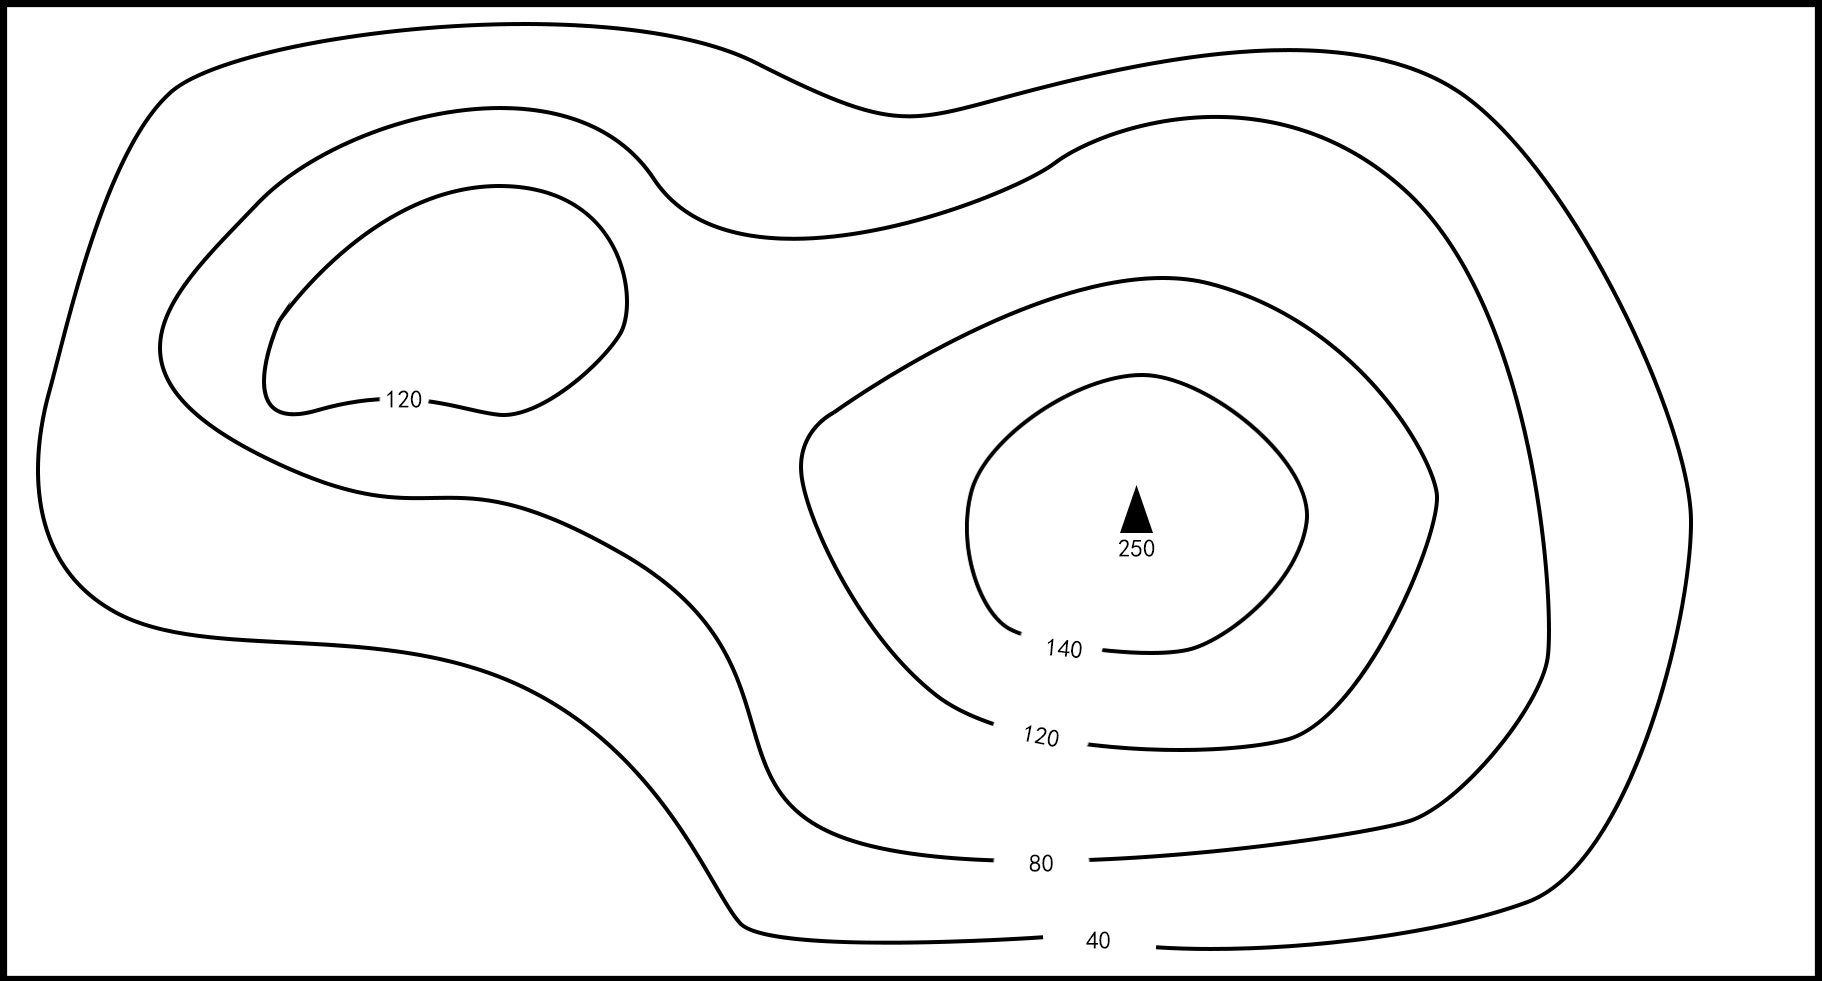
\includegraphics[width=0.75\textwidth]{/map-1/map-1}
  \caption{分层地形图}
  \label{fig:map-1}
\end{figure}

首先进行栅格化。

\begin{algorithm}[H]
  \caption{地图栅格化}\label{algorithm-grid}
  \KwData{原地图 $Map$, 栅格大小 $X$}
  \KwResult{栅格 $Grid$}

  $Grid$.Height $\leftarrow$ $ceil(Map.Length/X)$\;
  $Grid$.Width $\leftarrow$ $ceil(Map.Width/X)$\;
  \For{$i\leftarrow 1$ \KwTo $Grid$.Height}{
    \For{$j\leftarrow 1$ \KwTo $Grid$.Width}{
      $Grid$.creatSquare($i$,$j$,$X$)\;
      $Grid$.Data [$i$] [$j$] .Hight $\leftarrow$ maxOfMap($Map$,$i*X$,$(i+1)*X$,$j*X$,$(j+1)*X$)\;
    }
  }
  showPictures($Map$,$Grid$)\;
\end{algorithm}

\begin{figure}[H]
  \centering
  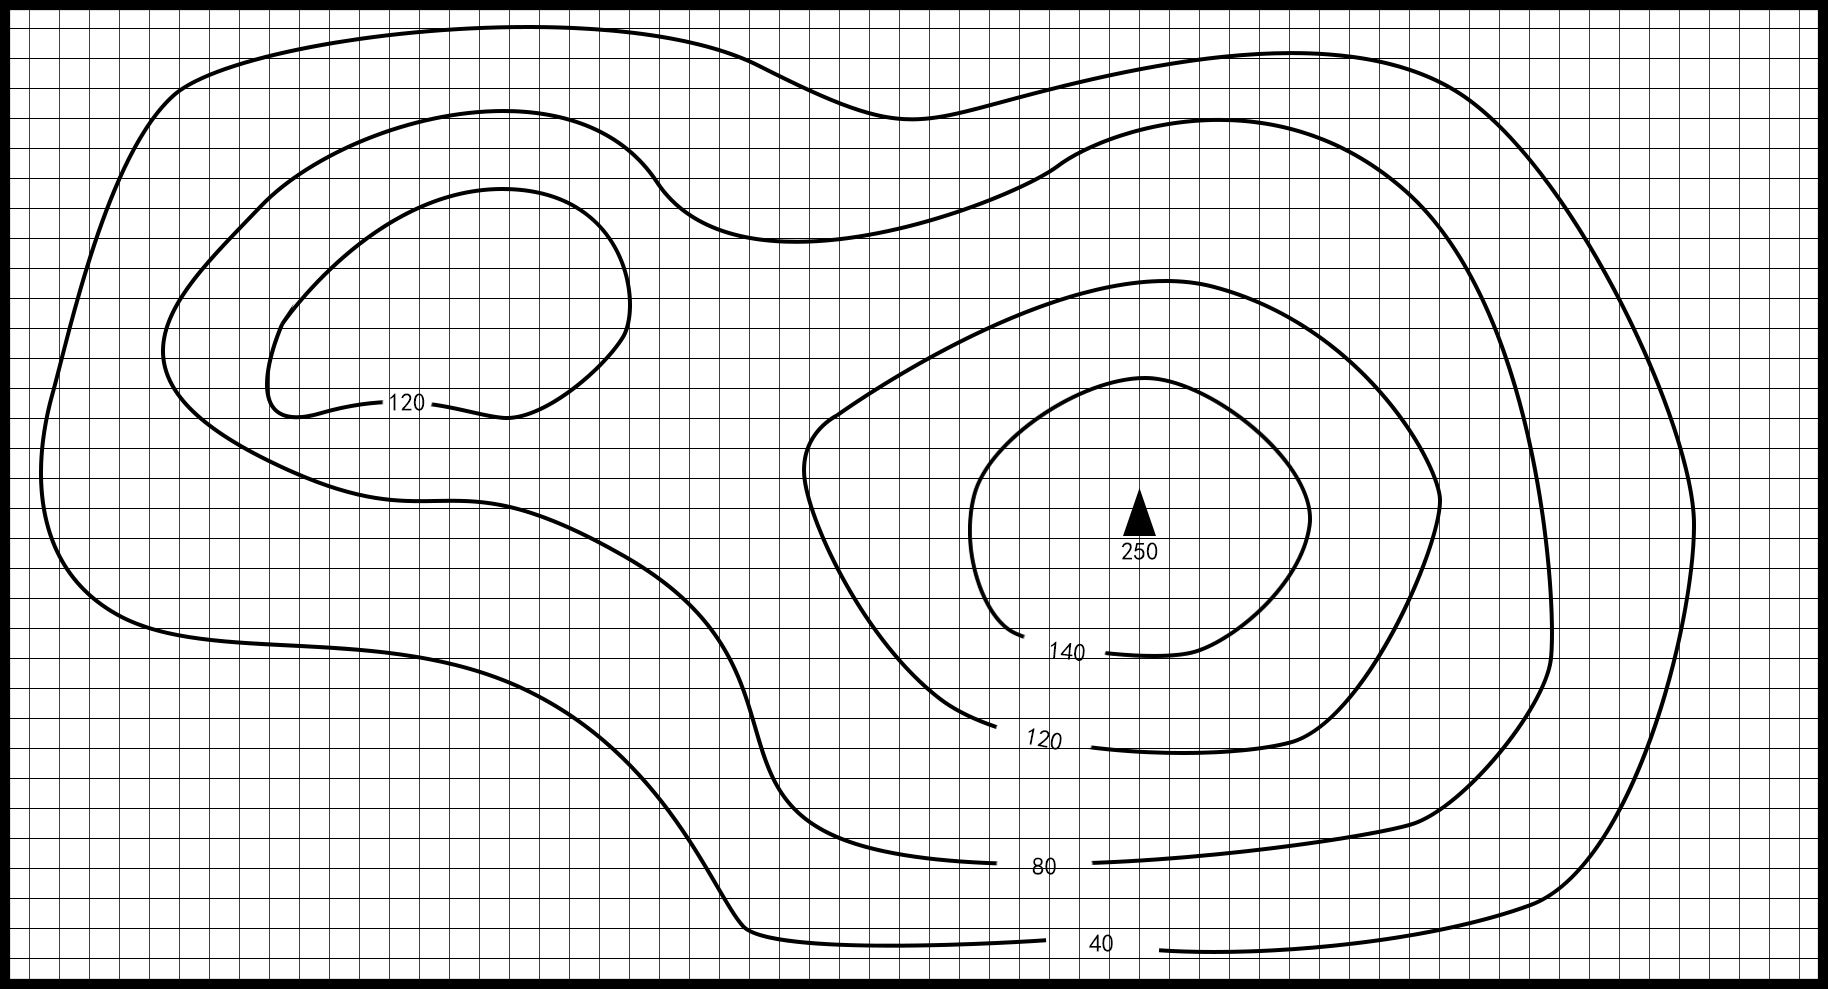
\includegraphics[width=0.75\textwidth]{/map-1/map-1-grid}
  \caption{栅格化后的地图}
  \label{fig:map-1-grid}
\end{figure}

之后以120m高度作为分界,
将栅格地图进行二值化处理:

\begin{algorithm}[H]
  \caption{地图栅格二值化}\label{algorithm-grid-noted}
  \KwData{原地图 $Map$, 栅格 $Grid$, 分界高度$HSet$}

  \For{$i\leftarrow 1$ \KwTo $Grid$.Hight}{
    \For{$j\leftarrow 1$ \KwTo $Grid$.Width}{
      \If{ $Grid$[$i$][$j$].Hight $>$ HSet}{
        Grid[$i$][$j$].RefuseFlag $\leftarrow$ $True$\;
        Grid[$i$][$j$].Color $\leftarrow$ $0x46831a$\;
        Grid[$i$][$j$].Alpha $\leftarrow$ $48$\;
      }
      \Else{
        Grid[$i$][$j$].RefuseFlag $\leftarrow$ $False$\;
        Grid[$i$][$j$].Color $\leftarrow$ $0x831a1a$\;
        Grid[$i$][$j$].Alpha $\leftarrow$ $48$\;
      }
    }
  }
  showPictures(Map,Grid)\;
\end{algorithm}

\begin{figure}[H]
  \centering
  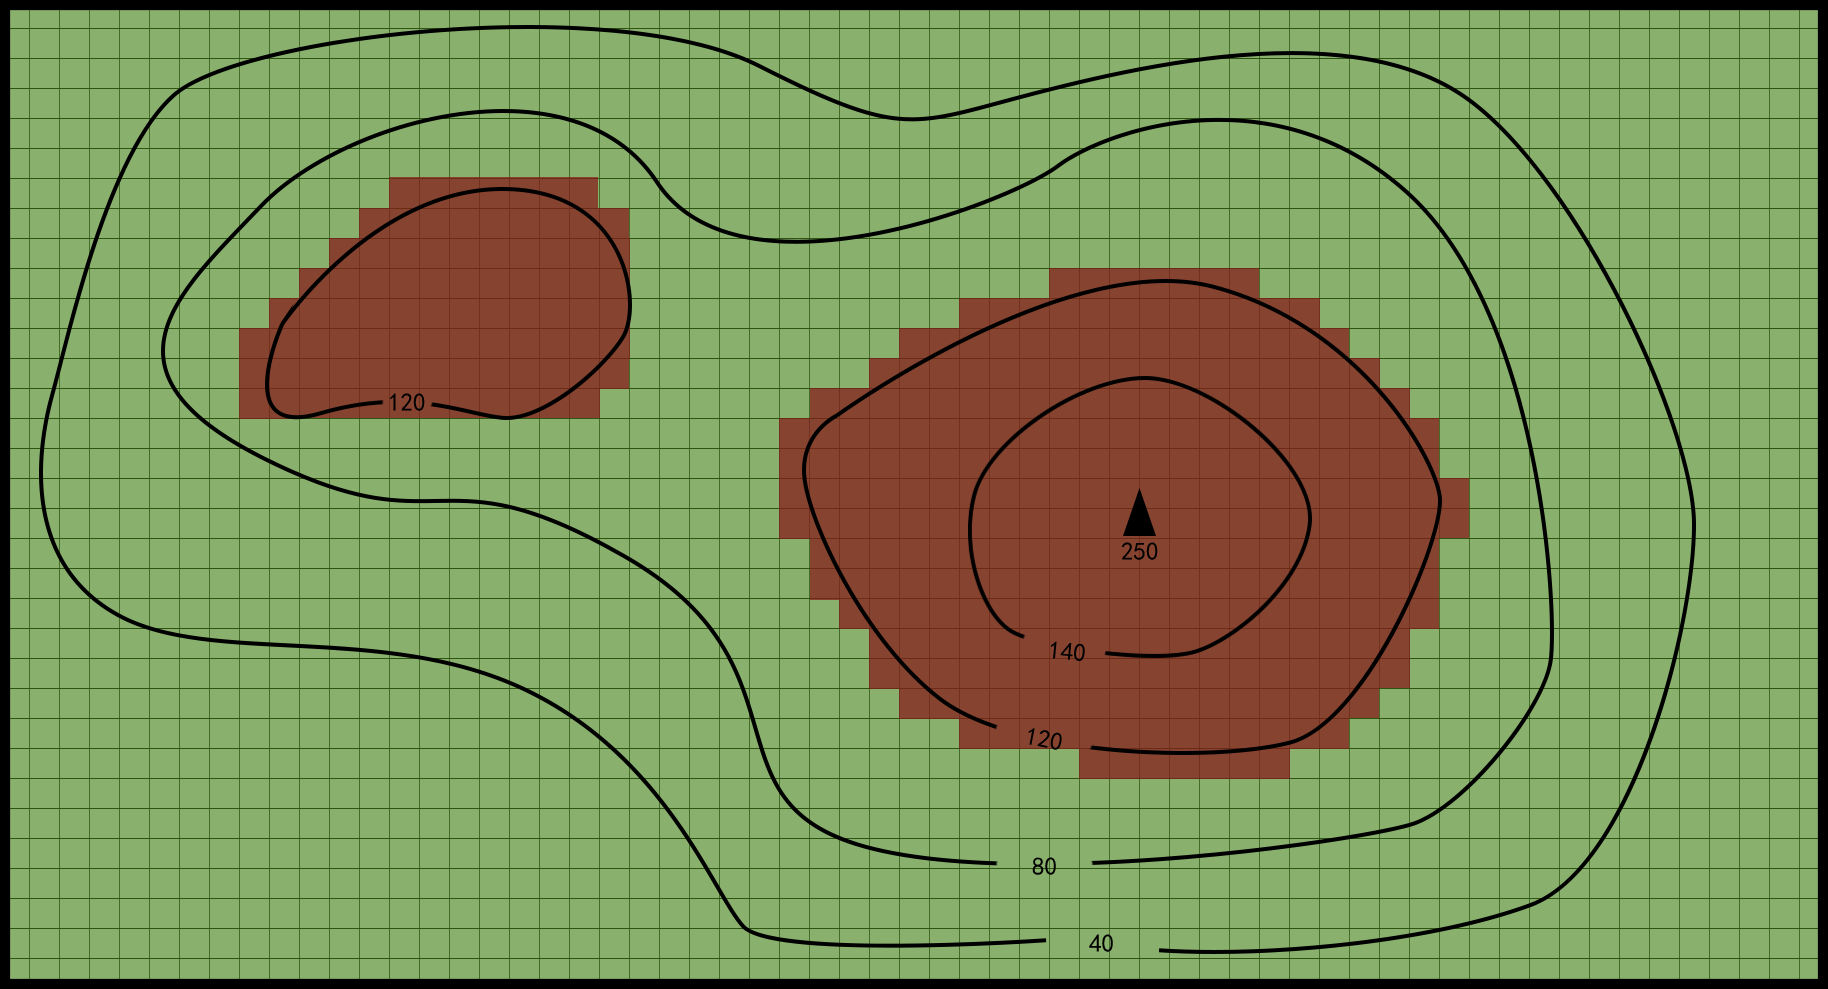
\includegraphics[width=0.75\textwidth]{/map-1/map-1-grid-noted}
  \caption{完成栅格法环境建模的地图}
  \label{fig:map-1-grid-noted}
\end{figure}

这样就完成了航迹图栅格化,即环境空间建模。
\subsection{图形法环境建模}
\subsubsection{图形法的概念}
图形法也是一种常用的环境建模方法,
通过将连续的空间离散化为非连续有限数量的点/块单元,
简化复杂环境的表示。
这种方法广泛应用于路径规划和导航领域,
尤其适用于二维且极广范围的建模。

图形法的核心思想是将环境划分为若干可通行点位,
并用道路连接,
每个道路用量值表示长度/耗时/代价等。
其本质为无向图。

图形法的优点同样在于其简单性和易于计算机存储与处理的特性,
并且可以大幅缩小问题规模。
\subsubsection{图形法的使用}
图形法环境建模有手动标记和自动识别两种方式。

手动标记即人工标记可通行点位并设置点间可通行道路,
输入计算机后自动处理。
自动识别一般使用四叉树算法等进行障碍物多边形化简化,
然后自动生成可通行点位并用道路连接。

本文使用手动标记法,
辅以自动处理程序完成图形法环境建模。
\subsubsection{实例分析与示例伪代码}
我们仍使用上一节栅格化时的分层地形图。

人工标记地图的可通行点位和道路:
\begin{figure}[H]
  \centering
  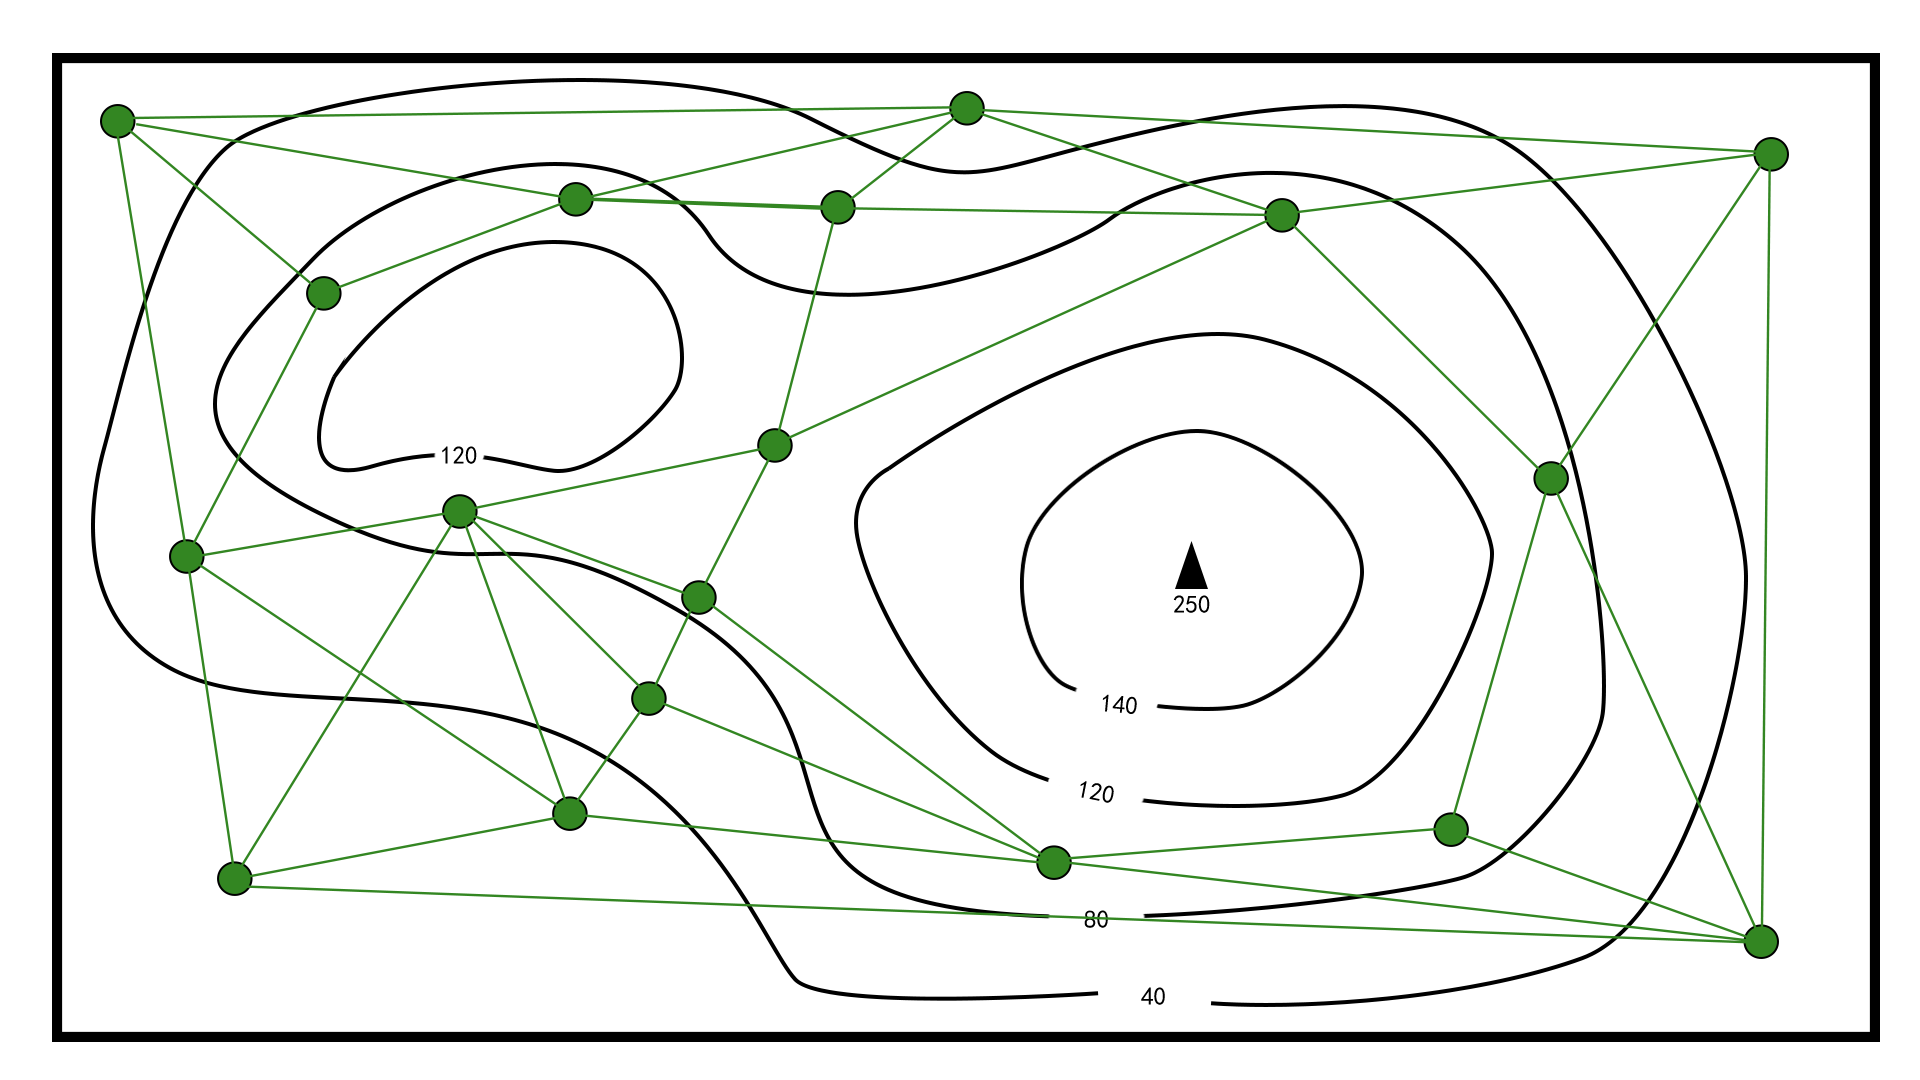
\includegraphics[width=0.75\textwidth]{/map-2/map-2-map}
  \caption{图形化后的地形图}
  \label{fig:map-2-map}
\end{figure}

利用自动处理程序将分散的点与路数据合并为一张无向图:

\begin{algorithm}[H]
  \caption{自动记录图形化地图}\label{algorithm-map-noted}
  \KwData{点集 $\bf{N}$, 路集 $R$}
  \KwOut{无向图 $D$}

  \For{$i\leftarrow 1$ \KwTo $N$.Num}{
    $D$.Dot.pushback($N$.Data[$i$])\;
  }
  \For{$i\leftarrow 1$ \KwTo $R$.Num}{
    $D$.Rd.newRoad($R$.Data[$i$].From,$R$.Data[$i$].To,$R$.Data[$i$].Value)\;
  }
\end{algorithm}

这样就完成了航迹图图形化,即环境空间建模。
%航迹规划算法-------------------------
\newpage\section{航迹规划算法与实现}
\subsection{传统基本航迹规划算法}
\subsubsection{概论}
传统基本航迹规划算法是基于搜索算法与最短路算法发展的,
属于计算机算法学中的图论部分。

其特点为:
基于数学分析,
处理速度较快,
约束条件较为单一(多仅考虑路径长度),
代码复杂度较小,
适合偏小规模且静态的问题,
且其最优解严格。

\subsubsection{模拟算法}
模拟算法严格上并不属于一种算法,
它是处理几种静态需求问题的方法,
例如矩形简单网格、多边形简单网格、矩形双重网格、环绕飞行等。

此处我们以矩形简单网格/2D往复式航迹规划方法作为实例演示模拟算法。

以哈尔滨工业大学二校区功夫菜园鸟瞰图为例:

\begin{figure}[H]
  \centering
  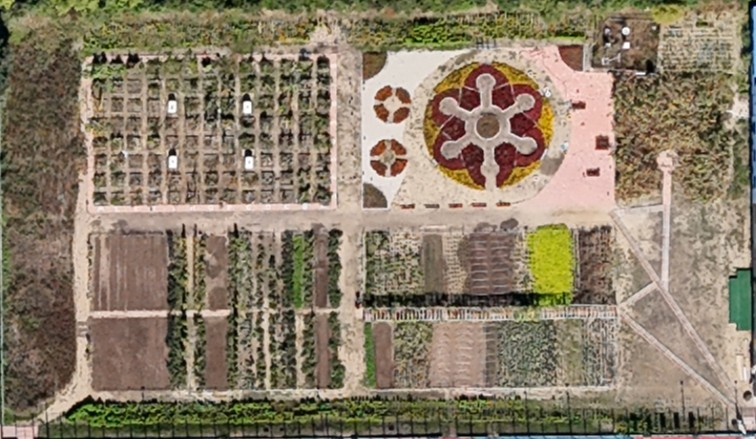
\includegraphics[width=0.75\textwidth]{/map-3/DJI_20250927104514_0043_D_Farm}
  \caption{功夫菜园鸟瞰图}
  \label{fig:map-3-farm}
\end{figure}

\begin{algorithm}[H]
  \caption{2D往复式航迹规划}\label{traditional-simulation}
  \KwData{地图(规划区) $Map$, 相邻航线间距 $D$, 转向区外延距离 $E$}
  \KwOut{航迹规划点集 $F$}

  $N$ $\leftarrow$ ceil($Map$.Width/$D$)\;
  \For{$i \leftarrow 0$ \KwTo $N-1$}{

    \If{$i\%2=0$}{

      \If{$i \ne 0$}{
        F.newPoint($Map$.Begin.La-$E$,$Map$.Begin.Lo+$i$*$D$)\;
      }
      F.newPoint($Map$.Begin.La,$Map$.Begin.Lo+i*$D$)\;
      F.newPoint($Map$.End.La,$Map$.Begin.Lo+i*$D$)\;
      \If{$i\ne N-1$}{
        F.newPoint($Map$.End.La+$E$,$Map$.Begin.Lo+$i$i*$D$)\;
      }

    }
    \Else{

      \If{$i\ne N-1$}{
        F.newPoint($Map$.End.La+$E$,$Map$.Begin.Lo+$i$i*$D$)\;
      }
      F.newPoint($Map$.End.La,$Map$.Begin.Lo+i*$D$)\;
      F.newPoint($Map$.Begin.La,$Map$.Begin.Lo+i*$D$)\;
      \If{$i \ne 0$}{
        F.newPoint($Map$.Begin.La-$E$,$Map$.Begin.Lo+$i$*$D$)\;
      }

    }
    
  }
\end{algorithm}

最终生成的航迹点集按先后顺序连直线在原地图上的情况:

\begin{figure}[H]
  \centering
  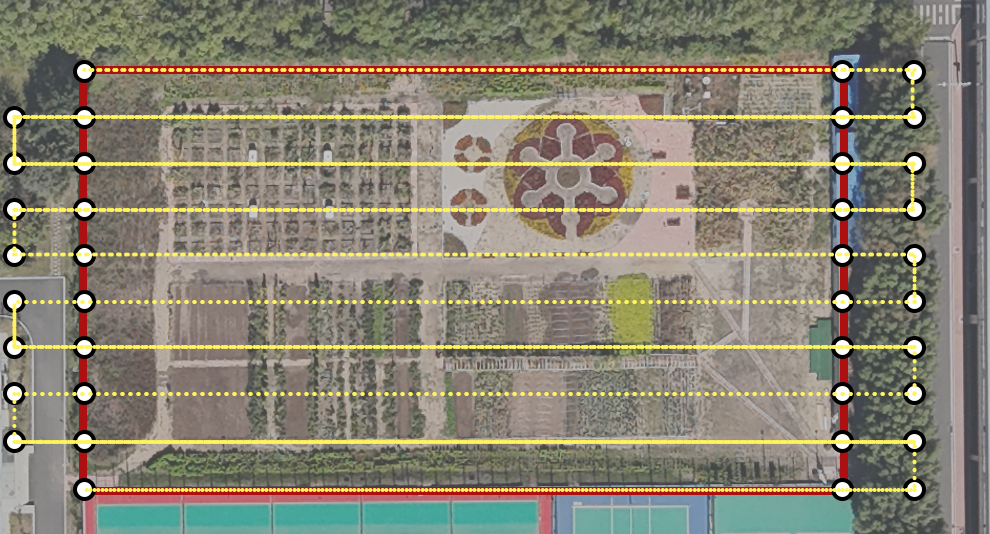
\includegraphics[width=0.75\textwidth]{/map-3/DJI_20250927104514_0043_D_Farm_Fin}
  \caption{功夫菜园鸟瞰图-航迹点图}
  \label{fig:map-3-farm-fin}
\end{figure}

\subsubsection{Dijkstra单源最短路算法}
Dijkstra单源最短路算法是荷兰计算机科学家 E.W.Dijkstra 发现的
一种用于求解非负权图上单个起点至单个终点的最短路径的算法。
事实上,
我们可以在相同时间内找到从给定源点到图中所有点的最短路径,
因此这个算法有时也被称为单源最短路径算法\textsuperscript{\cite{ref4}}。

对于一个有 $n$ 个点,
$m$ 条路的非负权图,
其朴素实现方法的时间复杂度为 $\mathcal{O}(n^2)$。
若使用其他数据结构处理该问题,
可以进一步降低时间复杂度。
如基于斐波那契堆的优化可做到 $\mathcal{O}(n \log n + m)$,
使用优先队列或线段树维护的做法可以达到 $\mathcal{O}(m \log n)$。
而目前理论最优实现为2025年6月15日,
由清华大学交叉信息院段然研究团队发现的针对无向图的,
不依赖于排序算法,
而是融合Dijkstra与Bellman-Ford两种最短路算法的实现方式。
其时间复杂度可缩小至 $\mathcal{O}(m \log ^{2/3} n)$\textsuperscript{\cite{ref5}}。
此时要根据图的疏密程度提前手动或解决过程中自动选择优化方式。

Dijkstra算法的核心过程如下:

\begin{algorithm}[H]
  \caption{Dijkstra单源最短路算法}\label{algorithm-traditional-Dijkstra}
  \KwData{点集 $\bf{T}$, 起点编号 $B$}
  \KwOut{已确定最短路长度的点集 $\bf{S}$}

  $Dis$[$0$ \KwTo $\bf{T}$.num] $\leftarrow$ 0\;
  $Dis$[$B$] $\leftarrow$ 0\;
  \While{$!T$.empty()}{
    $Next \leftarrow$ The point in $\bf{T}$ who have the confirmed shortest path.\;
    $S$.pushback($Next$)\;
    \For{$i \leftarrow 0$ \KwTo $Next$.RdNum}{
      $Dis$[$Next$.RoadData[$i$].To] $\leftarrow$ min($Dis$[$Next$.RoadData[$i$].To] , $Dis$[$Next$] $+$ $Next$.RoadData[$i$].Length)
    }
  }
\end{algorithm}

\subsubsection{IDA*搜索算法}
IDA*是一种混合了迭代加深算法与A*的搜索算法。
其中迭代加深算法是一种每次限制搜索深度(剪枝)的深度优先搜索(DFS)算法,
而A*搜索算法是一种在带权有向图上找到单个起点与终点之间的最短路径的改进广度优先搜索(BFS)算法。

由于IDA*使用了动态更新的剪枝阈值 $C$ 和估价函数 $h(x)$,
所以其没有严格数学证明下的 $\mathcal{O}$ 时间复杂度。

IDA*的主要实现过程:

设定起点 $s$,
估价函数 $h(x)$。

首先基于迭代加深搜索,
设定一个较小的搜索深度限制 $limit$ 与一个成本阈值 $C = h(s)$,
每次迭代搜索未得到答案时,
就将 $limit$ 增加 $1$ 并从头开始下一次迭代.

而在一次迭代中,
从起点 $s$ 开始进行深度优先搜索,
记录到达当前结点 $x$ 的实际成本 $g(x)$,
并利用它到终点的最小成本估计 $h(x)$进行剪枝。
如果沿着当前路径到达终点的总成本估计 
\[
  f(x) = g(x) +  h(x)
\]
超过限制 $C$,
则停止对该分支的搜索。

同时,
成本阈值 $C$ 将在两次迭代间进行更新。
每次迭代的分支因超限停止时,
就将所有尚未访问的后继结点的总成本估计的最小值记录下来。
本次迭代结束后,
将 $C$ 更改为记录的最小值,
然后继续下一轮迭代。

\subsection{现代智能航迹规划算法}
\subsubsection{概论}
现代智能航迹规划算法主要是基于智能优化与机器学习发展的。
由于其高并行性、实时性、强鲁棒性、自组织自学习等优点,
近年来已被广泛应用于复杂环境下的无人机自主航迹规划问题\textsuperscript{\cite{ref6}\cite{ref7}}。

其特点为:
基于智能优化与机器学习;
找到严格解处理速度偏慢,
但能够快速找到可行解;
代码复杂度较高;
可以有更多约束条件;
对动态问题具有更强的适应性;
解多为较优解,不为严格最优解。

同时由于其代码复杂度相较传统算法过高,
后续讨论算法实现时不再采用伪代码书写方式,
而是改为以语言描述其算法进行过程。
\subsubsection{遗传算法(Genetic Algorithm, GA)}
遗传算法是一类基于生物进化论和遗传学机理的随机搜索优化算法。

在进行规划时,
将初始的路径进行一次基因编码,
进行种群初始化,
然后根据任务约束构建适应度函数,
通过选择、交叉、变异等遗传算子开始逐代演化,
接着对种群个体进行评价,
除非满足终止条件,
否则继续进行演化过程,
最终得到最优航迹\textsuperscript{\cite{ref8}}。

但该算法的朴素实现存在后期局部搜索能力较差,
可能存在早熟性收敛、规划时间较长等缺点,
仍需在算法的各个过程中进行积极优化以得质量更高的算法。
\subsubsection{蚁群算法(Ant Colony Optimization, ACO)}
蚁群算法是一种基于自然界蚂蚁觅食行为的仿生算法。

该算法主要包括初始化参数、构建解空间、更新信息素与判断终止条件四步。

其核心思想来源于蚂蚁集群觅食的生物学现象。
形式化的,
该算法先限定每次迭代可遍历次数。
在每次迭代的每次遍历的前进过程中,
倾向于将新点放在原来点权更高的前进路径上。
\[
\text{路径的点权密度} ={ \sum_{i=1}^{\text{该路径各点}}{\text{点}i\text{的权重}} } / \text{路径长度}
\]
每次迭代结束时,
将所有已放置点的权重统一减弱。
由于每次的新增点均倾向于更优路径,
且旧点随时间消逝,
所以该算法产生的点集将随迭代次数增加愈发趋近于最优解(最短路)。
\subsubsection{灰狼算法(GWO)}
灰狼算法是一种模仿灰狼在捕猎、围猎以及攻击猎物过程中的自然行为的算法,
其利用位置更新和信息传递来进行全局最优解的搜索\textsuperscript{\cite{ref9}}。

与蚁群算法一步一步由起点导向终点不同,
灰狼算法是先随机生成一定数量的随机解,
并设定一个适应度函数,
然后进入迭代状态:
先利用适应度函数找到目前解中三个最优的解,
然后以此三个最优解为参考调整其余解,
且调整幅度随迭代次数的增加而减小。
如此反复迭代若干次后,
所有解基本都聚集在最优解附近,
此时我们选取其中最优的一条即为一个可行最优解\textsuperscript{\cite{ref10}}。

同时由于其搜索过程中总是追随三个临时最优解,
朴素的灰狼算法极其容易陷入局部最优解。
所以我们可以通过修改部分过程,
例如:
调整幅度不再线性随迭代次数变化,
而是改为动态调整的非线性规划;
以及不止向最优解调整,
同时向最优解的镜像位置进行探索,
扩大搜索范围防止过早陷入局部最优解等。
此时我们称该算法为改进灰狼算法(IGWO)。
\subsubsection{布谷鸟搜索算法(Cuckoo Search, CS)}
布谷鸟算法是一种参考布谷鸟特殊的寄生繁殖习性进行的算法。
其依靠智能随机游走和强制更新机制来寻找最优路径。

布谷鸟算法在优胜劣汰方面与遗传算法略有相似,
而初始解的生成与灰狼算法相似,
但布谷鸟算法的实现过程与它们有极大差别。
并且布谷鸟算法还依赖一种名为"莱维飞行"的模式:
大多数时间在当前位置附近进行小范围密集搜索以进行局部精细优化;
而小概率的进行一次远距离跳跃,
在一个陌生区域重新开始搜索。

布谷鸟算法的具体实现过程如下:

首先初始化若干可行解,
设置一个弃巢概率常数与适应度函数,
然后进入迭代优化循环:

先依次进行"莱维飞行"调整解。

然后利用适应度函数比较调整前后解的优劣,
保留更优解。

最后挑出随机或最劣的一部分解,
直接丢弃并生成新的解。

如此迭代循环,
所有解的平均质量会越来越高,
整体也就越来越接近最优解。

布谷鸟算法的大幅跳跃与丢弃解行为,
使其在搜寻全局最优解而不陷入局部最优解上有极大优势。
但这也导致其在精细化路径时难以快速优化现有路径。
所以该算法大多时候会作为先导处理算法,
与其他算法(如IGWO)结合以提高处理精度与速率。
\subsection{多算法混合与优化}
以上提到的与其他尚未提及的各种算法均有各自的优势区域,
也有不足之处。
此时,多算法结合的优化成为了新选择。

比如在蚁群算法步进时采用A*算法改进前进选择过程;
或者结合布谷鸟算法与改进灰狼算法,
提高前期全局最优解被找到的概率,
并保证后续路径精细化时的精度与速率。
我们通过将各个函数放在各自擅长的处理位置,
进一步提高了求解速度。

这种混合算法已成为当前最短路算法/路径规划算法的热门研究方向,
未来我们或许能将更多的算法融合在一起,
打造出来时间复杂度更低甚至允许单机在线自动规划路径的算法。
%航迹平滑算法-------------------------
\newpage\section{航迹平滑算法}
\subsection{航迹平滑概论}
航迹平滑,
是指将航迹规划算法生成的路线中,
对于无人机难以实现的路径(如直角,锐角等),
或者为了利于航空拍摄效果更顺滑,
通过平滑/曲线化处理,
使其航线更加合理的一种操作。
\subsection{三次样条插值法(Cubic Spline Interpolation, Spline插值)}
三次样条插值法是多项式插值法在最高次项为三次时的算法。
经过三次插值后位置曲线是平滑的,
保证了路径形状的可行性。

参考\cite{ref11}中的解决方案,
对于 $n$ 个航迹点,
通过依次进行四个步骤:\\
参数化、建立方程、求解三对角方程组和样条系数、生成平滑航迹方程。

我们就可以得到一条平滑的曲线航迹,
使无人机可以平滑飞行。

\subsection{贝塞尔曲线法(Bézier Curve)}
相较于Spline插值,
贝赛尔曲线法的计算过程更为简单。

我们两两进行三次贝塞尔曲线连接。
对于 $n$ 个航迹点 $Q_n$,
我们先计算每一个点的切线方向向量 $T_i$,
\begin{equation}
  \begin{cases}
    T_0 = Q_1 - Q_0 ,\\
    T_i = (Q_{i+1}-Q_{i-1})/2 , 1 \leq i \leq n-2 ,\\
    T_{n-1} = Q_{n-1} - Q_{n-2}
  \end{cases}
  \nonumber
\end{equation}

然后我们将切线向量归一化处理:
\[ T_{i_{normal}} = T_i / \lvert {\lvert T_i \rvert}\rvert \]

而三次贝塞尔连接需要四个点(起点,终点,两个控制点),
所以我们需要计算出每两点间的两个控制点。

对于 $Q_i$ 到 $Q_{i+1}$,
\begin{equation}
  \begin{cases}
    d_i=\sqrt{(x_{i+1}-x_i)^2 + (y_{i+1}-y_i)^2} ,\\
    P_{1_x} = x_i + \alpha \cdot d\cdot T_{i_{{normal}_x}} ,\\
    P_{1_y} = y_i + \alpha \cdot d\cdot T_{i_{{normal}_y}} ,\\
    P_{2_x} = x_{i+1} - \beta \cdot d\cdot T_{{i+1}_{{normal}_x}} ,\\
    P_{2_y} = y_{i+1} - \beta \cdot d\cdot T_{{i+1}_{{normal}_y}}
  \end{cases}
  \nonumber
\end{equation}
其中 $\alpha$ 和 $\beta$ 是张力参数,
一般取 $1/3$。

最后,
我们利用两点及对应生成两控制点生成平滑点,
组成平滑曲线:
\begin{equation}
  \begin{cases}
    t \in (0,1) ,\\
    x(t) = (1-t)^3\cdot x_i + 3\cdot (1-t)^2\cdot t\cdot P_{1_x} + 3\cdot(1-t)\cdot t^2\cdot P_{2_x}+t^3\cdot x_{i+1} ,\\
    y(t) = (1-t)^3\cdot y_i + 3\cdot (1-t)^2\cdot t\cdot P_{1_y} + 3\cdot(1-t)\cdot t^2\cdot P_{2_y}+t^3\cdot y_{i+1}
  \end{cases}
  \nonumber
\end{equation}

这样我们便完成了利用贝赛尔曲线法的航迹平滑化操作。
%航迹平滑算法-------------------------
\newpage\section{结论}
本文依次讨论了航迹规划中环境空间建模、航迹规划、航迹平滑化三个步骤。
这三个步骤目前都有较为成熟的算法解决方案,
但仍可被改进以图更高的问题处理效率与答案质量。

未来随着公路桥梁数目的进一步增多,
无人机自动航迹规划方法将大幅度地提高工作效率,
方便建设工作与后续日常维护。
并且,
我们可以不拘泥于单架无人机,
而是采取多机编队,
进行机组航迹规划,
利用并行工作指数级地提高工作速度,
而这将对无人机硬软件与航迹规划算法提出更高的要求与挑战。

目前,
大多数论文提出的航迹算法仍然停留在虚拟仿真环境中,
而没有进入实际验证与使用阶段。
以后的算法研究不应该是孤立的,
而是要结合大模型、分布式云管理等先进技术,
并将算法真正的运用到实际中去,
切实测试算法的性能、可靠性与优缺点,
助力无人机技术进一步发展,
推动我国桥梁事业向未来大步迈进。
%参考文献库--------------------------------------------------------
\newpage\section{参考文献}\begin{thebibliography}{20}
\bibitem{ref1}中华人民共和国交通运输部. 2024年交通运输行业发展统计公报[R/OL]. (2025-06-12)[2025-10-04]. https://xxgk.mot.gov.cn/2020/jigou/zhghs/202506/t20250610\_4170228.html.
\bibitem{ref2}欧林联. 无人机自动化巡检在城市桥梁运维中的探索和应用[J]. 福建建设科技, 2025,(05):97-100. DOI:CNKI:SUN:FJJK.0.2025-05-024.
\bibitem{addref1}Aabid Abdul, Parveez Bisma, Parveen Nagma, et al. Reviews on Design and Development of Unmanned Aerial Vehicle (Drone) for Different Applications[J]. Journal of Mechanical Engineering Research and Developments. (2022).45.53-69.
\bibitem{ref3}王硕, 李洋, 赵蕴龙, 等. 无人机航迹规划算法综述[J/OL]. 哈尔滨工程大学学报, 1-14[2025-10-04]. https://link.cnki.net/urlid/23.1390.U.20250616.1544.003.
\bibitem{ref4}Javaid, Muhammad Adeel. Understanding Dijkstra's Algorithm[R/OL]. (2013-04-10)[2025-10-18]. DOI:10.2139/ssrn.2340905.
\bibitem{ref5}Ran Duan, Jiayi Mao, Xiao Mao, et al. 2025.Breaking the Sorting Barrier for Directed Single-Source Shortest Paths[R/OL]. (2025-06-15)[2025-10-18] In Proceedings of the 57th Annual ACM Symposium on Theory of Computing (STOC '25). Association for Computing Machinery, New York, NY, USA, 36–44. DOI:10.1145/3717823.3718179
\bibitem{ref6}Zhao Y J, Zheng Z, Liu Y. Survey on Computational-Intelligence-Based UAV Path Planning[J]. Knowledge-Based Systems, 2018, 158:54-64.
\bibitem{ref7}郭启敏, 张鹏, 王应洋, 等. 无人机自主航迹规划智能算法综述[J]. 航空兵器,2023,30(3):29-40. DOI:10.12132/ISSN.1673-5048.2022.0220 
\bibitem{ref8}黄磊, 鞠训光, 吴潇轩, 等. 基于遗传算法的无人机航迹规划[J]. 计算机科学与应用, 2020,10(5):1034-1043. DOI:10.12677/csa.2020.105107
\bibitem{ref9}赵桐. 无人机航迹智能规划算法研究[D]. 长春工业大学,2025. DOI:10.27805/d.cnki.gccgy.2025.001166.
\bibitem{ref10}王永琦, 江潇潇. 基于混合灰狼算法的机器人路径规划[J]. 计算机工程与科学, 2020, 42(07): 1294-1301.
\bibitem{ref11}McKinley S, Levine M. Cubic spline interpolation[J]. College of the Redwoods, 1998, 45(1): 1049-1060.
\end{thebibliography}
%原创性声明-------------------------
\newpage\section{原创性声明}
~\\
~\\
本人郑重声明:

所呈交的结课报告/论文是我个人在小组合作与导师指导下进行研究工作所取得的成果。
尽我所知,
除了文中注明之处外,
该报告/论文中不包含其他个人、集体或组织已经发表或撰写过的研究成果,
与我一同合作的组员对本文及研究内容所做的任何贡献将在后文致谢部分中作明确的说明并表示谢意。

作者签名:

日期:\qquad 年\qquad 月\qquad 日
%致谢-------------------------
\newpage\section{致谢}
感谢导师李顺龙老师和郭亚鹏老师,
他们开展的《无人机摄像及应用》(TS22505)课程使我受益匪浅。
我学到了很多新的知识,
了解到了无人机摄像过程中的各种问题与解决方案,
还见到了许许多多的新兴路径规划算法。

同时感谢王安东老师,
他与前述两位老师一起负责了实操课的教学,
采用多种方式助力我们练习无人机飞行与拍摄活动。
最后他们还拿出了实验室的大疆经纬M300无人机给我们体验飞行,
这是一次及其难忘的崭新体验。
并且他在本文撰写期间无私地给予了许多指导与建议,
再次感谢。
~\\

我作为该课程2025秋季班第三组的小组长,
在此感谢我的五位组员。
他们分工合力迅速完成了另一份课程报告(《图像的三维重构》)的撰写,
为我减轻了许多负担。

同时,
在本文撰写过程中,
他们也给予了我许多鼓励与支持,
再次感谢他们。
~\\

在此,
我列举出所有的小组成员,
他们分别是(组员排名不分先后):

\qquad 组长\quad 刘宇轩\quad 25L0212\quad 2025112195

\qquad 组员\quad 何家震\quad 25L0502\quad 2025110903

\qquad 组员\quad 刘一诺\quad 25L0205\quad 2025111917

\qquad 组员\quad 张芮嘉\quad 25L0209\quad 2025111819

\qquad 组员\quad 石艾琳\quad 25L0207\quad 2025112232

\qquad 组员\quad 齐露雅\quad 25L0216\quad 2025111932
~\\

感谢我的父亲母亲,
在我忙于报告撰写时,
他们谅解了我对他们的忽视,
并且给予了我无条件的爱与支持。

本结课报告的顺利完成,
离不开上述的每一位老师、同学和亲人的鼎力相助,
他们的贡献是本文不可或缺的基石。
~\\

最后,
再次郑重地感谢以上所有人。


%附录-------------------------
\newpage\section{附录}
《Understanding Dijkstra's Algorithm》. Javaid, Muhammad Adeel. 

电子版详稿请参考 https://doi.org/10.2139/ssrn.2340905

纸质版请参考下文(无图与表):
~\\

《理解 Dijkstra 算法》

Muhammad Adeel Javaid

CompTIA 成员供应商咨询委员会

{\bf 摘要:}
Dijkstra 算法(以其发现者 E.W. Dijkstra 命名)解决了在图中从一个点(源点)到目标点寻找最短路径的问题。事实上,我们可以在相同时间内找到一个给定源点到图中所有点的最短路径,因此该问题有时也被称为单源最短路径问题。本文将借助简单易懂的示例和图示,帮助您理解 Dijkstra 算法的基础概念。

{\bf 引言:}
虽然像网络设计师和分析师这样的人需要对 Dijkstra 算法有透彻的理解,但对于我们其他人来说,进行一次简单而仔细的考察就足够了。我们不必以分步形式列出算法,而是直接来看一个示例求解过程。我们示例的目标是,在下图中找到从节点 A 到其他每个节点的最低成本路由。

[图 1]

首先,您需要创建一个表,如表 10-2(a)(下方所示),表中为除起始节点 A 之外的网络中的每个节点设置一列。该表还需要包含一个名为"已访问"的列,您将在此列出每个已被访问过的节点。更准确地说,当您在此列中列出一个节点时,表示您已经到达该节点并检查了该节点的所有直接邻居。此外,该表应包含一个名为"下一跳"的最后行,用于指示数据包离开节点 A 后应遍历的下一个节点(仅指下一个节点)。例如,如果节点 G 列下的"下一跳"值为 B,那么一个离开节点 A 且目的地为节点 G 的数据包,下一步应被传输到节点 B。在处理此示例时,您应记住,该算法的工作方式是,此表一旦完成(参见本节末尾的表 10-2(h)),仅显示从节点 A 到其他每个节点应进行的下一跳。就本示例而言,这意味着一旦您到达节点 B(在前往节点 G 的途中),您将需要查阅一个不同的表——即节点 B 的 Dijkstra 表——以确定下一跳。

[表 10-2(a) Dijkstra 算法初始表]

创建表格后,选择起始节点 A,访问它,并将起始节点添加到"已访问"列表中,如表 10-2(b) 所示。之后,定位节点 A 的每个直接邻居(仅一个链路或一跳之遥的节点)且该邻居尚未在"已访问"列表中。计算从节点 A 到这些邻居中每一个的旅行成本,并将这些值填入表中。例如,节点 B 距离节点 A 一跳,尚未被访问,从 A 到 B 的旅行成本为 2 个单位。在这种情况下,您应在表 10-2(b) 的节点 B 列中输入 2,以表示从节点 A 到节点 B 的路径成本,并在"下一跳"行中输入 B,注明要到达 B,您将在下一跳直接前往 B。您也可以从 A 到 C 一跳,成本为 4,"下一跳"值为 C;从 A 到 D 一跳,成本为 5,"下一跳"值为 D。这些值也记录在表 10-2(b) 中。请注意,我们尚未"访问"B、C 或 D。我们只访问了 A,并且我们仅仅检查了 A 与 B、A 与 C 以及 A 与 D 之间的链路成本。

[表 10-2(b) 访问节点 A 后的 Dijkstra 算法表]

没有更多节点是 A 的直接邻居,并且节点 A 的所有直接邻居链路都已被检查,因此您需要选择下一个要访问的节点。根据算法,下一个要访问的节点必须是当前表中成本最低的节点。因此,您必须选择节点 B。通过指定选择成本最低的下一个节点,该算法将在所有情况下找到最低成本。定位节点 B 的尚未被访问的直接邻居(目前只有 A 被访问),并确定从节点 A 经由节点 B 到节点 B 的每个直接邻居的旅行成本。请注意,节点 A 已被访问,因此您应在此阶段将其排除在考虑范围之外(没有必要走回头路)。节点 B 的尚未被访问的直接邻居是 D、E 和 G。从节点 A 经由节点 B 到节点 D 的成本是 4(从 A 到 B 的链路成本为 2,从 B 到 D 的链路成本为 2)。由于此成本小于直接从 A 到 D 的成本(如表 10-2(b) 所示,为 5),因此用新值 4 替换原值 5,以更新表格。此更新在表 10-2(c) 中高亮显示。您还应将节点 D 列下"下一跳"行中的 D 替换为 B,因为从节点 A 到节点 D 的新的最低成本路径现在始于数据包离开节点 A 后首先前往节点 B。

[表 10-2(c) 访问节点 A 和 B 后的 Dijkstra 算法表]

从 A 经由 B 到 E 的成本是 6 (2 + 4),从 A 经由 B 到 G 的成本是 9 (2 + 7)。分别在 E 和 G 列中输入值 6 和 9,如表 10-2(d) 所示。B 也是 E 和 G 的"下一跳"值。

[表 10-2(d) 访问节点 A 和 B 后的 Dijkstra 算法表,续]

接下来让我们访问节点 C,因为正如您在表 10-2(d) 中看到的,它具有下一个最小的成本。C 的尚未被访问的直接邻居是 F 和 G。从 A 经由 C 到 F 的成本是 7 (4 + 3)。在 F 列中输入值 7,在"下一跳"行中输入值 C,如表 10-2(e) 所示。从节点 A 经由 C 到 G 的旅行成本是 9 (4 + 5)。由于这个新值 9 不小于表 10-2(d) 中的当前值(也是 9),因此在这种情况下无需更新表格。

[表 10-2(e) 访问节点 A、B 和 C 后的 Dijkstra 算法表]

接下来让我们访问节点 D,因为它具有下一个最小的成本。D 的尚未被访问的直接邻居是 E、F 和 G。从 A 经由 D(经由 B)到 E 的成本是 5 (4 + 1)。由于此值小于从 A 到 E 的当前成本(小于 6),通过在 E 列中输入 5 来更新表格(参见表 10-2(f) 作为参考)。我们仍然在离开 A 后首先前往 B 才能到达 E,因此"下一跳"行中的值 B 不会改变。从 A 经由 D 到 F 的成本是 10 (5 + 5)。从 A 经由 D 到 G 的成本也是 10。因为已输入 F 和 G 列中的值小于 10(换句话说,表格已经反映了这些节点的最低成本路径),所以您不需要更新表格。

[表 10-2(f) 访问节点 A、B、C 和 D 后的 Dijkstra 算法表]

下一个要访问的节点是 E。E 的尚未被访问的直接邻居是 G。从节点 A 经由节点 E(经由 D 经由 B)到节点 G 的旅行成本是 7 (2 + 2 + 1 + 2)。这条路径的成本 7 小于已填入 G 列中的值,因此您应该用这个新的、更小的值替换表中的当前值,如表 10-2(g) 所示。

[表 10-2(g) 访问节点 A、B、C、D 和 E 后的 Dijkstra 算法表]

下一个要访问的节点是 F。F 的尚未被访问的唯一直接邻居是 G。从节点 A 经由 F(经由 C)到节点 G 的旅行成本是 8。此成本不小于 F 的当前值,因此不更新表格。

最后一个要访问的节点是 G。但是,G 没有尚未被访问的直接邻居,因此我们完成了。

表 10-2(h) 显示了最终结果。从这个表中,您现在可以轻松查找从节点 A 到任何其他节点的最低成本路径。如果数据包源自节点 A 并且目的地是节点 x,路由器中的软件将简单地查阅表的 x 列以确定数据包下一步应前往何处。要找到从另一个节点开始的最低成本路由,您需要再次应用 Dijkstra 算法。例如,如果您希望找到从节点 C 到任何其他节点的最低成本路径,您将通过以节点 C 作为起始位置重复最低成本算法来生成一个新表。

[表 10-2(h) 从节点 A 开始的七节点子网应用 Dijkstra 算法的结果]

Dijkstra 算法为每个节点 j 分配一对标签 (pj, dj),其中 pj 是在从节点 1 到 j 的现有最短路径上位于节点 j 之前的节点,dj 是该最短路径的长度。一些标签被称为临时的,即它们在后续步骤中可能会改变;一些标签被称为永久的,即它们是固定的,并且从节点 1 到被永久标记的节点的最短路径已被找到。

我们用 djk 表示弧 (j,k) 

步骤 1. 用永久标签 (Ø,0) 标记节点 1。用临时标签 (1, d1j) 标记每个满足 (1,j) 是图中一条弧的节点 j。用临时标签 (Ø,∞) 标记图中所有其他节点。

步骤 2. 令 j 是一个具有最小标签 dj 的临时标记节点,即 dj=min{dl: 节点 l 是临时标记的}。对于每个满足 (j,k) 在图中存在的节点 k,如果 dk > dj + djk,则按如下方式重新标记 k:pk=j, dk=dj+djk。节点 j 的标签视为永久的。

步骤 3. 重复步骤 2,直到图中所有节点都被永久标记。通过读取标签 pj 可以找到最短路径。示例。 找到从节点 1 到所有其他节点的最短路径。我们将具有永久标签的节点标为红色。从节点 1 到所有其他节点的最短路径:

{\bf Dijkstra 算法示例}

已知:一个网络拓扑图 G,包含 6 个节点,节点间的链路成本如下所示:

求解:使用 Dijkstra 算法寻找从节点 A 到 F 的最低成本路径

解答:

令 T = {A, B, C, D, E, F} = 网络中的节点数

s = 源节点 = A

N = 迄今为止已处理的节点集合

c(i,j) = 如果两个节点直接连接,则为从节点 i 到节点 j 的链路成本。

= ∞ 如果 i 和 j 之间没有链路

D(v) = 当前已知的从节点 s 到节点 v 的最短路径(最低成本路径)的成本。当算法终止时,D(v) 是网络中从源点 s 到目的地 v 的最短路径的成本。

P(v): 从源点 s 到 v 的路径上的前驱节点,即紧接在 v 之前的节点

1) [初始化]

N = {A} 初始化集合 N 包含源节点 A
计算 v 属于集合 T 但不属于集合 N 的 D(v)。
需要计算 v = B, C, D, E, F 的 D(v)

2) [获取下一个节点]

找到不在 N 中且 D(w) 最小的 w。即上一步中最小的 D(w),将该节点 w 添加到集合 N 中。如果相等,则随机选取其中一个。
本例中,D(D) = 1 是最小的,因此我们将节点 w = D 添加到集合 N。
N = { A, D }

3) [更新最短路径成本]

D(v) = min [ D(v), D(w) + c(w,v) ] 对于所有不在 N 中的节点 v
= min [ D(v), D(D) + c(D,v) ] 对于节点 v = B, C, E, F

4) [获取下一个节点]

找到不在 N 中且 D(w) 最小的 w。即上一步中最小的 D(w),将该节点 w 添加到集合 N 中。如果相等,则随机选取其中一个。
本例中,D(E) 和 D(B) 具有相同的最小成本 2,我们随机选取一个。我们选择节点 w = E 加入集合 N。
N = { A, D, E }

5) [更新最短路径成本]

D(v) = min [ D(v), D(w) + c(w,v) ] 对于所有不在 N 中的节点 v
= min [ D(v), D(E) + c(E,v) ] 对于节点 v = B, C, F

6) [获取下一个节点]

找到上一步中最小的 D(v),将该节点添加到 N。如果相等,随机选取其中一个。
D(B) 的成本最低 = 2。我们选择节点 w = B 加入集合 N。
N = { A, D, E, B }

7) [更新最短路径成本]

D(v) = min [ D(v), D(w) + c(w,v) ] 对于所有不在 N 中的节点 v
= min [ D(v), D(B) + c(B,v) ] 对于节点 v = C, F

8) [获取下一个节点]

找到上一步中最小的 D(v),将该节点添加到 N。如果相等,选取其中任意一个。
D(C) 是最小的,因此我们将节点 w = C 添加到集合 N。
N = { A, D, E, B, C}

9) [更新最短路径成本]

D(v) = min [ D(v), D(w) + c(w,v) ] 对于所有不在 N 中的节点 n
= min [ D(v), D(C) + c(C,v) ] 对于节点 n = F

10) [获取下一个节点]

找到上一步中最小的 D(v),将该节点添加到 N。如果相等,选取其中任意一个。
D(F) 是唯一剩下的节点,因此我们将节点 w = F 添加到集合 N。
N = { A, D, E, B, C, F }
N = T,因此算法终止。

11) 现在,我们需要写出从节点 A 到所有其他节点的最短路径。从后往前写,因为这些是到达各节点的最短路径成本,然后反向追溯到源节点 A。D(v) 列是从源节点 A 到 v 的最短路径成本。
\end{document}